%%%%%%%%%%%%%%%%%%%%%%%%%%%%%%%%%%%%%%%%%%%%%%%%%%%%%%%%%%%%%%%%%%%%%%%%%%%%%%%%%%
\begin{frame}[fragile]\frametitle{Idea}
\begin{center}

\includegraphics[width=0.3\linewidth,keepaspectratio]{midcurve18}

Can Large Language Models ``learn'' the dimension reduction transformation?
\end{center}	
\end{frame}


%%%%%%%%%%%%%%%%%%%%%%%%%%%%%%%%%%%%%%%%%%%%%%%%%%%%%%%%%%%%%%%%%%%%%%%%%%%%%%%%%
\begin{frame}[fragile]\frametitle{}
\begin{center}
{\Large LLMs for Midcurve Implementation}
\end{center}
\end{frame}

%%%%%%%%%%%%%%%%%%%%%%%%%%%%%%%%%%%%%%%%%%%%%%%%%%%%%%%%%%%%%%%%%%%%%%%%%%%%%%%%%%
\begin{frame}[fragile]\frametitle{Proposed Approach}

Text to Text Transformation Learning:

\begin{itemize}
\item Geometric Representation: A text-based representation of the geometry/graph/network will be explored to leverage Natural Language Processing (NLP) techniques.
\item Existing Methods: The paper (Fatemi, Halcrow, and Bryan 2023) surveys several text-based representations for graph data, but none appear specifically suited for geometric shapes.
\item Proposed Approach: A geometry representation similar to 2D Boundary Representation (B-rep) will be utilized, adapting the concept from 3D to 2D.
\end{itemize}	

\end{frame}

%%%%%%%%%%%%%%%%%%%%%%%%%%%%%%%%%%%%%%%%%%%%%%%%%%%%%%%%%%%%%%%%%%%%%%%%%%%%%%%%%%
\begin{frame}[fragile]\frametitle{Representation of Geometry}


\begin{itemize}
\item One limitation of 2D geometry-shape, represented as a sequential list of points, is that we can not represent line intersections or concentric loops. 
\item To address this a more comprehensive structure has been proposed which is based on the corresponding 3D structure popular in Solid Modeling, called Brep (Boundary Representation).
\end{itemize}	

\end{frame}

%%%%%%%%%%%%%%%%%%%%%%%%%%%%%%%%%%%%%%%%%%%%%%%%%%%%%%%%%%%%%%%%%%%%%%%%%%%%%%%%%%
\begin{frame}[fragile]\frametitle{2D Brep Representation}

Leverage a geometry representation similar to that found in 3D B-rep (Boundary representation), but in 2D. It can be shown as:

\begin{lstlisting}
{
 'ShapeName': 'I',
 'Profile': [(5.0, 5.0), (10.0, 5.0), (10.0, 20.0), (5.0, 20.0)],
 'Midcurve': [(7.5, 5.0), (7.5, 20.0)],
 'Profile_brep': {
    'Points': [(5.0, 5.0), (10.0, 5.0), (10.0, 20.0),(5.0, 20.0)], # list of (x,y) coordinates
    'Lines': [[0, 1], [1, 2], [2, 3], [3, 0]], # list of point ids (ie index in the Points list)
                'Segments': [[0, 1, 2, 3]] # list of line ids (ie index in Lines list)
    },
 'Midcurve_brep': {
    'Points': [(7.5, 5.0), (7.5, 20.0)],
    'Lines': [[0, 1]],
                'Segments': [[0]]
    },    
}
\end{lstlisting}	
\end{frame}

%%%%%%%%%%%%%%%%%%%%%%%%%%%%%%%%%%%%%%%%%%%%%%%%%%%%%%%%%%%%%%%%%%%%%%%%%%%%%%%%%%
\begin{frame}[fragile]\frametitle{Data}

         \begin{center}
	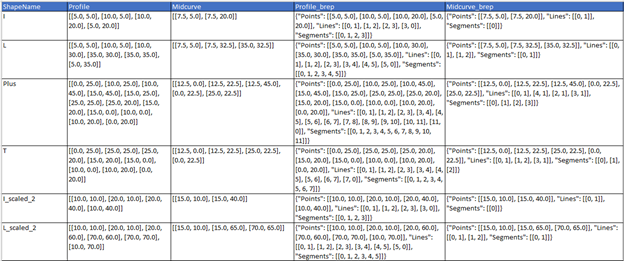
\includegraphics[width=\linewidth]{images/shapes_csv}
	\label{fig_csv}
    \end{center}
	
\end{frame}


%%%%%%%%%%%%%%%%%%%%%%%%%%%%%%%%%%%%%%%%%%%%%%%%%%%%%%%%%%%%%%%%%%%%%%%%%%%%%%%%%%
\begin{frame}[fragile]\frametitle{Data Explanation}

Column information is as below:

\begin{itemize}
\item ShapeName (text): name of the shape. Just for visualization/reports.
\item Profile (text): List of Points coordinates (x,y) representing outer profile shape, typically closed.
\item Midcurve (text): List of Points coordinates (x,y) representing inner midcurve shape, typically open.
\item Profile\_brep (text): Dictionary in Brep format representing outer profile shape, typically closed.
\item Midcurve\_brep (text): Dictionary in Brep format representing inner midcurve shape, typically open.
\end{itemize}	

Each Segment is a continuous list of lines. In case of, say `Midcurve-T`, as there is an intersection, we can treat each line in a separate segment. In the case of 'Profile O', there will be two segments, one for outer lines and another for inner lines. Each line is a list of points, for now, linear. Points is a list of coordinates (x,y), later can be (x,y,z).

\end{frame}

%%%%%%%%%%%%%%%%%%%%%%%%%%%%%%%%%%%%%%%%%%%%%%%%%%%%%%%%%%%%%%%%%%%%%%%%%%%%%%%%%%
\begin{frame}[fragile]\frametitle{Data Resolution}

\begin{itemize}
\item Once we have this Brep representations of both, profile and the corresponding midcurve, in the text form, then we can try various machine translation approaches or LLM based fine tuning or few-shots prompt engineering.
\item One major advantage of text based method over image based method is that image output still has stray pixels, cleaning which will be a complex task. But the text method has exact points. It may just give odd lines, which can be removed easily.
\end{itemize}	


\end{frame}

%%%%%%%%%%%%%%%%%%%%%%%%%%%%%%%%%%%%%%%%%%%%%%%%%%%%%%%%%%%%%%%%%%%%%%%%%%%%%%%%%
\begin{frame}[fragile]\frametitle{}
\begin{center}
{\Large Prompt based techniques}
\end{center}
\end{frame}


%%%%%%%%%%%%%%%%%%%%%%%%%%%%%%%%%%%%%%%%%%%%%%%%%%%%%%%%%%%%%%%%%%%%%%%%%%%%%%%%%%
\begin{frame}[fragile]\frametitle{Few Shots Prompt}
\begin{lstlisting}
You are a geometric transformation program that transforms input 2D polygonal profile to output 1D polyline profile. Input 2D polygonal profile is defined by set of connected lines with the format as: ...

Below are some example transformations, specified as pairs of 'input' and the corresponding 'output'. After learning from these examples, predict the 'output' of the last 'input' specified.
Do not write code or explain the logic but just give the list of lines with point coordinates as specified for the 'output' format.

input:[((5.0,5.0), (10.0,5.0)), ... ((5.0,35.0), (5.0,5.0))]
output: [((7.5,5.0), (7.5, 32.5)), ... ((35.0, 32.5) (7.5, 32.5))]

input: [((5,5), (10, 5)), ...  (5, 20)), ((5, 20),(5,5))]
output: [((7.5, 5), (7.5, 20))]

:
input:[((0, 25.0), (25.0,25.0)),...  ((0,20.0),(0, 25.0))]
output:
\end{lstlisting}	
\end{frame}

%%%%%%%%%%%%%%%%%%%%%%%%%%%%%%%%%%%%%%%%%%%%%%%%%%%%%%%%%%%%%%%%%%%%%%%%%%%%%%%%%%
\begin{frame}[fragile]\frametitle{Few Shot Examples Shapes}
The first input example above represents ‘L’ shape (shown below) and the second is an ‘I’, whereas the 3rd is a ‘Plus’ sign shape.

\begin{center}
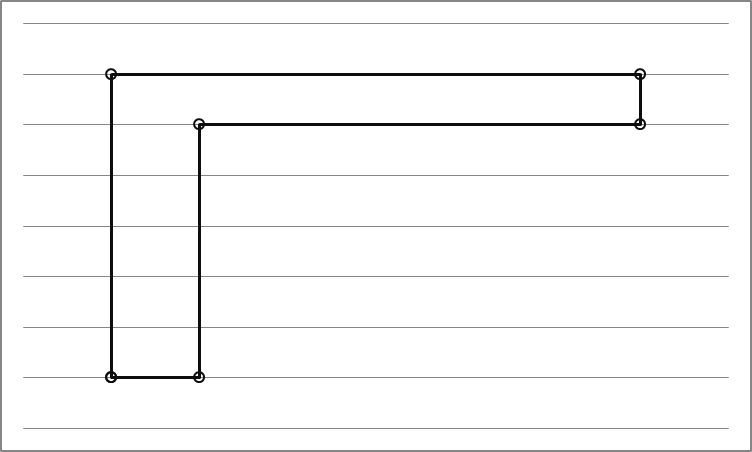
\includegraphics[width=\linewidth,keepaspectratio]{L}
\end{center}	
\end{frame}

%%%%%%%%%%%%%%%%%%%%%%%%%%%%%%%%%%%%%%%%%%%%%%%%%%%%%%%%%%%%%%%%%%%%%%%%%%%%%%%%%%
\begin{frame}[fragile]\frametitle{Few Shot Examples Shapes}
The last shape for which LLM has been asked for the answer is actually a ‘T’ shape. The picture below shows the correct/actual answer as well.

\begin{center}
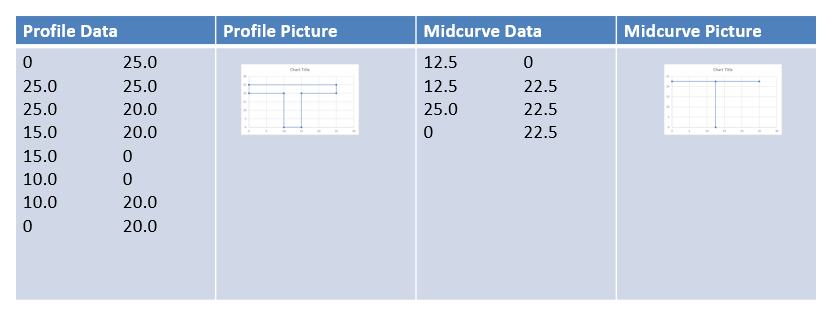
\includegraphics[width=\linewidth,keepaspectratio]{T}
\end{center}	
\end{frame}

%%%%%%%%%%%%%%%%%%%%%%%%%%%%%%%%%%%%%%%%%%%%%%%%%%%%%%%%%%%%%%%%%%%%%%%%%%%%%%%%%%
\begin{frame}[fragile]\frametitle{Output}
And the outputs computed by various LLMs (ChatGPT, Perplexity AI, Bard) , along with the real/actual answer:

\begin{lstlisting}
Actual: [((12.5,0), (12.5,22.5)), ((12.5,22.5),(25.0,22.5)), ((12.5,22.5),(0,22.5))]
ChatGPT: [((2.5, 0), (2.5, 22.5)), ((2.5, 22.5), (2.5, 45.0)), ((2.5, 22.5), (25.0, 22.5)), ((2.5, 22.5), (12.5, 22.5)), ((2.5, 22.5), (0, 22.5)), ((2.5, 22.5), (25.0, 22.5))]
Perplexity: [((12.5,0), (12.5, 22.5)), ((12.5, 22.5),(12.5,45.0)), ((12.5, 22.5), (0,22.5)), ((12.5, 22.5), (25.0,22.5))]
Bard: [((12.5, 0), (12.5, 25.0)), ((12.5, 25.0), (25.0, 25.0)), ((25.0, 25.0), (25.0, 0))]
\end{lstlisting}	
\end{frame}

%%%%%%%%%%%%%%%%%%%%%%%%%%%%%%%%%%%%%%%%%%%%%%%%%%%%%%%%%%%%%%%%%%%%%%%%%%%%%%%%%%
\begin{frame}[fragile]\frametitle{Output}

Visually here is how results from different LLMs look:

\begin{center}
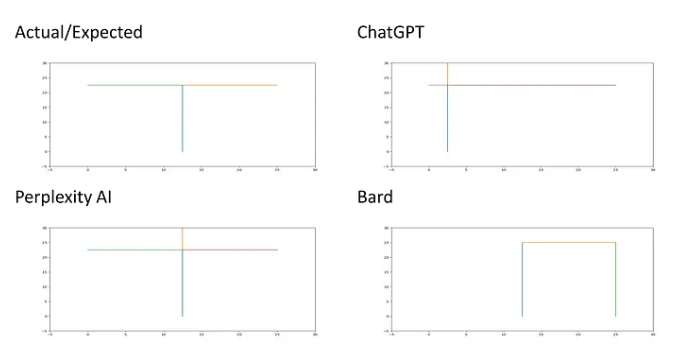
\includegraphics[width=\linewidth,keepaspectratio]{midcurve34}
\end{center}	
\end{frame}

%%%%%%%%%%%%%%%%%%%%%%%%%%%%%%%%%%%%%%%%%%%%%%%%%%%%%%%%%%%%%%%%%%%%%%%%%%%%%%%%%%
\begin{frame}[fragile]\frametitle{Interpretation}

All of the above have failed. Even latest, the results are:
\begin{itemize}
\item \lstinline|llama 7B g4_0 ggml: (8, 17) & (64, 32)|: Wrong.
\item \lstinline|Bard: [((8.33,5),(8.33, 22.5)), ((8.33, 22.5), (25,22.5)), ((8.33, 22.5), (0,25))]|: Wrong.
\item \lstinline|Hugging Chat: [((12.5, 0), (12.5, 22.5)), ((12.5, 22.5), (25.0, 22.5)), ((25.0, 22.5), (25.0, 25.0))]|: a bit wrong on the last line
\item \lstinline|GPT-4: [((12.5,0), (12.5,22.5)), ((12.5,22.5),(0,22.5)), ((12.5,22.5),(25.0,22.5))]| just change in sequence of lines, and that's inconsequential, so the answer is correct.
\end{itemize}	
\end{frame}

%%%%%%%%%%%%%%%%%%%%%%%%%%%%%%%%%%%%%%%%%%%%%%%%%%%%%%%%%%%%%%%%%%%%%%%%%%%%%%%%%%
\begin{frame}[fragile]\frametitle{Interpretation}

LLMs by an large seem to have failed for such simple shapes.

There could be two prominent reasons:

\begin{itemize}
\item The prompt design was not effective and could be improved upon.
\item The LLM model itself is not able to learn the pattern and predict well.
\end{itemize}	

The current geometry representation as a sequence of lines, has limitations. Trying to look for a good representation to store geometry/graph/network as text so that NLP (Natural Language Techniques) can be applied.
\end{frame}

%%%%%%%%%%%%%%%%%%%%%%%%%%%%%%%%%%%%%%%%%%%%%%%%%%%%%%%%%%%%%%%%%%%%%%%%%%%%%%%%%
\begin{frame}[fragile]\frametitle{}
\begin{center}
{\Large Fine-tuning based techniques}
\end{center}
\end{frame}


%%%%%%%%%%%%%%%%%%%%%%%%%%%%%%%%%%%%%%%%%%%%%%%%%%%%%%%%%%%%%%%%%%%%%%%%%%%%%%%%%%
\begin{frame}[fragile]\frametitle{Training Data}

\begin{lstlisting}[basicstyle=\tiny, breaklines=true, breakatwhitespace=true,label=lst:python]
from datasets import load_dataset, Dataset, DatasetDict

base_url = "/content/drive/MyDrive/ImpDocs/Work/AICoach/Notebooks/data/"
dataset = load_dataset("csv", data_files={"train": base_url + "midcurve_llm_train.csv",
                                          "test": base_url + "midcurve_llm_test.csv",
                                          "validation": base_url + "midcurve_llm_val.csv"})
DatasetDict({
    train: Dataset({
        features: ['ShapeName', 'Profile', 'Midcurve', 'Profile_brep', 'Midcurve_brep'],
        num_rows: 793
    })
    test: Dataset({
        features: ['ShapeName', 'Profile', 'Midcurve', 'Profile_brep', 'Midcurve_brep'],
        num_rows: 99
    })
    validation: Dataset({
        features: ['ShapeName', 'Profile', 'Midcurve', 'Profile_brep', 'Midcurve_brep'],
        num_rows: 100
    })
})

\end{lstlisting}

\end{frame}

%%%%%%%%%%%%%%%%%%%%%%%%%%%%%%%%%%%%%%%%%%%%%%%%%%%%%%%%%%%%%%%%%%%%%%%%%%%%%%%%%%
\begin{frame}[fragile]\frametitle{Data Preprocessing}

The dataset is used to fine-tune the base model called ``Salesforce/codet5-small''. Trained model is saved and used for inference on test samples.

\begin{lstlisting}[basicstyle=\tiny, breaklines=true, breakatwhitespace=true,label=lst:python]
from transformers import T5ForConditionalGeneration, AdamW, get_linear_schedule_with_warmup
import pytorch_lightning as pl

class CodeT5(pl.LightningModule):
    def __init__(self, lr=5e-5, num_train_epochs=15, warmup_steps=1000):
        super().__init__()
        self.model_name = "Salesforce/codet5-small"
        self.model = T5ForConditionalGeneration.from_pretrained(self.model_name)
        self.save_hyperparameters()
        
    def forward(self, input_ids, attention_mask, labels=None):
        outputs = self.model(input_ids=input_ids, attention_mask=attention_mask, labels=labels)
        return outputs        
        :
        :

model = CodeT5()

trainer = Trainer(max_epochs=5,accelerator="auto",# gpus=1,
                  default_root_dir="/content/drive/MyDrive/CodeT5/Notebooks/Checkpoints",
                  logger=wandb_logger,
                  callbacks=[early_stop_callback, lr_monitor])
trainer.fit(model)
\end{lstlisting}

\end{frame}

%%%%%%%%%%%%%%%%%%%%%%%%%%%%%%%%%%%%%%%%%%%%%%%%%%%%%%%%%%%%%%%%%%%%%%%%%%%%%%%%%%
\begin{frame}[fragile]\frametitle{Inferencing}

The output predicted far away from the corresponding ground truth. 

There could be many reasons for the mismatch such as the quality of LLM, training parameters, and above all, need for a far bigger dataset for fine-tuning. But overall, the approach and preliminary results look promising to warrant further investigations.

\begin{lstlisting}[basicstyle=\tiny, breaklines=true, breakatwhitespace=true,label=lst:python]
input_ids = tokenizer(test_example['Profile_brep'], return_tensors='pt').input_ids
outputs = model.generate(input_ids)

print("Ground truth:", test_example['Midcurve_brep'])
print("Generated Midcurve:", tokenizer.decode(outputs[0], skip_special_tokens=True))

Ground truth: "{\"Points\": [[-8.4, 3.28], [-20.68, -5.33]], \"Lines\": [[0, 1]], \"Segments\": [[0]]}"
Generated Midcurve: "{\"Points\": [[-8.83, 4.32], [-21.23
\end{lstlisting}

\end{frame}